\subsection{Abuse Detection}
Abuse detection is a single-class classification problem. The challenge is to detect when a comment from a conversation would be considered insulting to another participant in the conversation. The idea is to create a generalisable classifier that can operate in near real-time. Classification is a form of supervised learning; it takes a set of data ${X, Y}$ where $X$ is a set of attributes and $Y$ is the target class. The goal is to model $Y$ as a function of $X$, $y = f(x)$, where $x \in X$ is a specific sample and $y \in Y$ is the corresponding class for that sample.

Abuse detection is primarily implemented in Python, consisting of multiple scripts. The script requires Python version 2.7 or above to executes due to certain dependencies and functions used. The script makes use of multiple Python libraries including Sci-kit learn \cite{scikit:home}, NLTK \cite{nltk}, Numpy \cite{Numpy} and Pandas \cite{Pandas}, and others such as MySQL, which provide machine learning models and objects for loading and processing the data. The code for this functionality has been modularised and is thus split across various files and classes. This allows modules to be included, instantiated, upgraded and reused whenever necessary.

\subsubsection{Data Description}
As mentioned previously, classification is a form of supervised learning. This means that a dataset is required to train the classifier which can then be used to make predictions on unseen instances. A suitable dataset was found online, provided by Impermium and hosted on the popular machine learning competitions site Kaggle \cite{Kaggle:Dataset}. The dataset was split into two files, \emph{train.csv} and \emph{test.csv}, and consisted of three attributes: Insult, Date, Comment. The training set contains 3,948 samples whereas the test set contains 2,648 samples.


\subsubsection{Data Preprocessing}
As the data has been downloaded from a third-party, we must ensure that it is in the correct format. The data preprocessing stage will ensure that all training and test data is consistent with the data we expect on the social network. This step is only carried during the training phase.

 The dataset was loaded into memory as a table (DataFrame) using the Pandas library. The library provides a function to read CSV files with headers as demonstrated in figure \ref{fig:AbuseDetection_LoadData}. A generic function was created for loading in the dataset as this functionality is required multiple times, for loading the test and training datasets separately.

\begin{figure}[H]
    \centering
    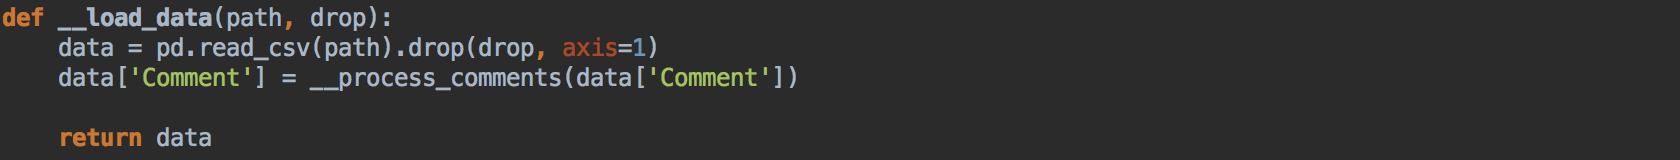
\includegraphics[width=\textwidth]{Images/Implementation/DataProcessing/AbuseDetection/LoadData}
    \caption{Loading in CSV data files.}
    \label{fig:AbuseDetection_LoadData}
\end{figure}

The raw dataset contains multiple errors which will affect the accuracy of the resulting model. As a result, before the data can be used, it needs to be processed and cleaned. For example, there are comments which contain several ASCII characters that have been encoded. Similarly, there are several comments which contain underscores and new line characters that must be stripped so features from the comments can be extracted correctly.

\begin{figure}[H]
    \centering
    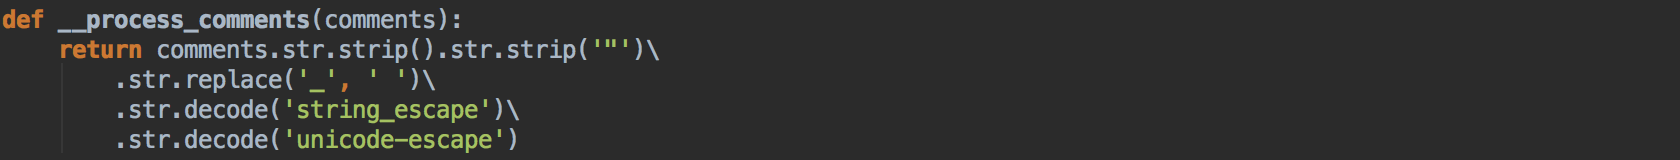
\includegraphics[width=\textwidth]{Images/Implementation/DataProcessing/AbuseDetection/ProcessComments}
    \caption{Function for processing comments and removing unnecessary characters.}
    \label{fig:AbuseDetection-ProcessComments}
\end{figure}

The function in figure \ref{fig:AbuseDetection-ProcessComments} processes the entire DataFrame, firstly removing any white space surrounding text, then replacing all the underscores with spaces. The resulting string is first decoded using \emph{string\_escape}, which produces a string that is suitable for use as a string literal. The string is then decoded again, but this time using \emph{unicode\_escape}, which produces a string that is suitable as Unicode literal \cite{Python:Codes}.

\begin{figure}[H]
    \centering
    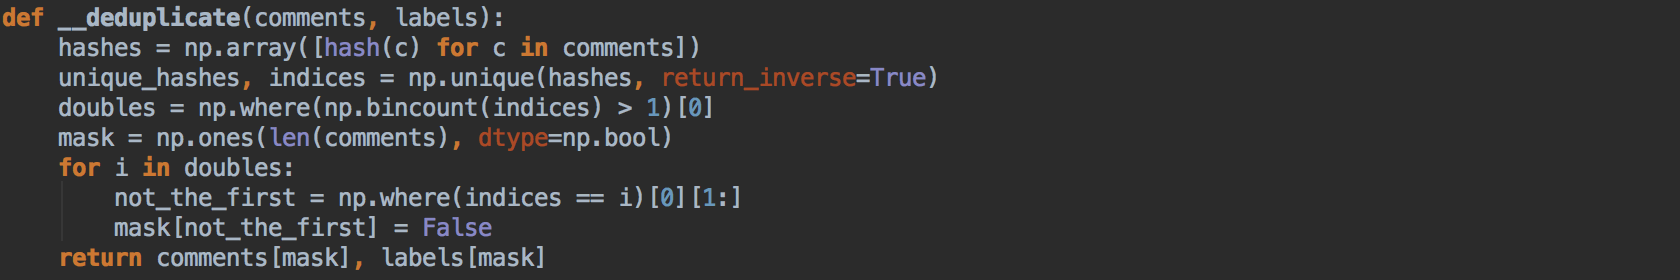
\includegraphics[width=\textwidth]{Images/Implementation/DataProcessing/AbuseDetection/Deduplicate}
    \caption{Function for removing duplicate comments.}
    \label{fig:AbuseDetection-Deduplicate}
\end{figure}

The next step involved removing any duplicate comments in the training set. The function in figure \ref{fig:AbuseDetection-Deduplicate} takes a set of comments and their labels to filter out duplicated comments, returning only unique comments with their associated labels. The first part of this process computes the hash of every comment. This will result in the same hash for two comments that are identical, due to the nature of the hashing process. Next, we take the indices of all the unique hashes, which returns bins containing the indices corresponding to every hash value. As a result, if a hash appears twice then it will contain two indices in its bin. The indices of the hashes are then used to find the duplicates where the bin has more than two indices in it. Given all the duplicates, we can generate a mask which only returns one instance of every duplicate comment. Finally, the mask is used to access all the unique comments and their associated labels.

\subsubsection{Feature Engineering} \label{sec:feature-engineering}
The raw data, a sequence of symbols, cannot be fed directly to the algorithms as most of them expect numerical feature vectors with a fixed size rather than the raw text documents with variable length \cite{scikit:tfidf}. In order to achieve a reasonable accuracy, the features of the dataset must be transformed into something meaningful.

\begin{figure}[H]
    \centering
    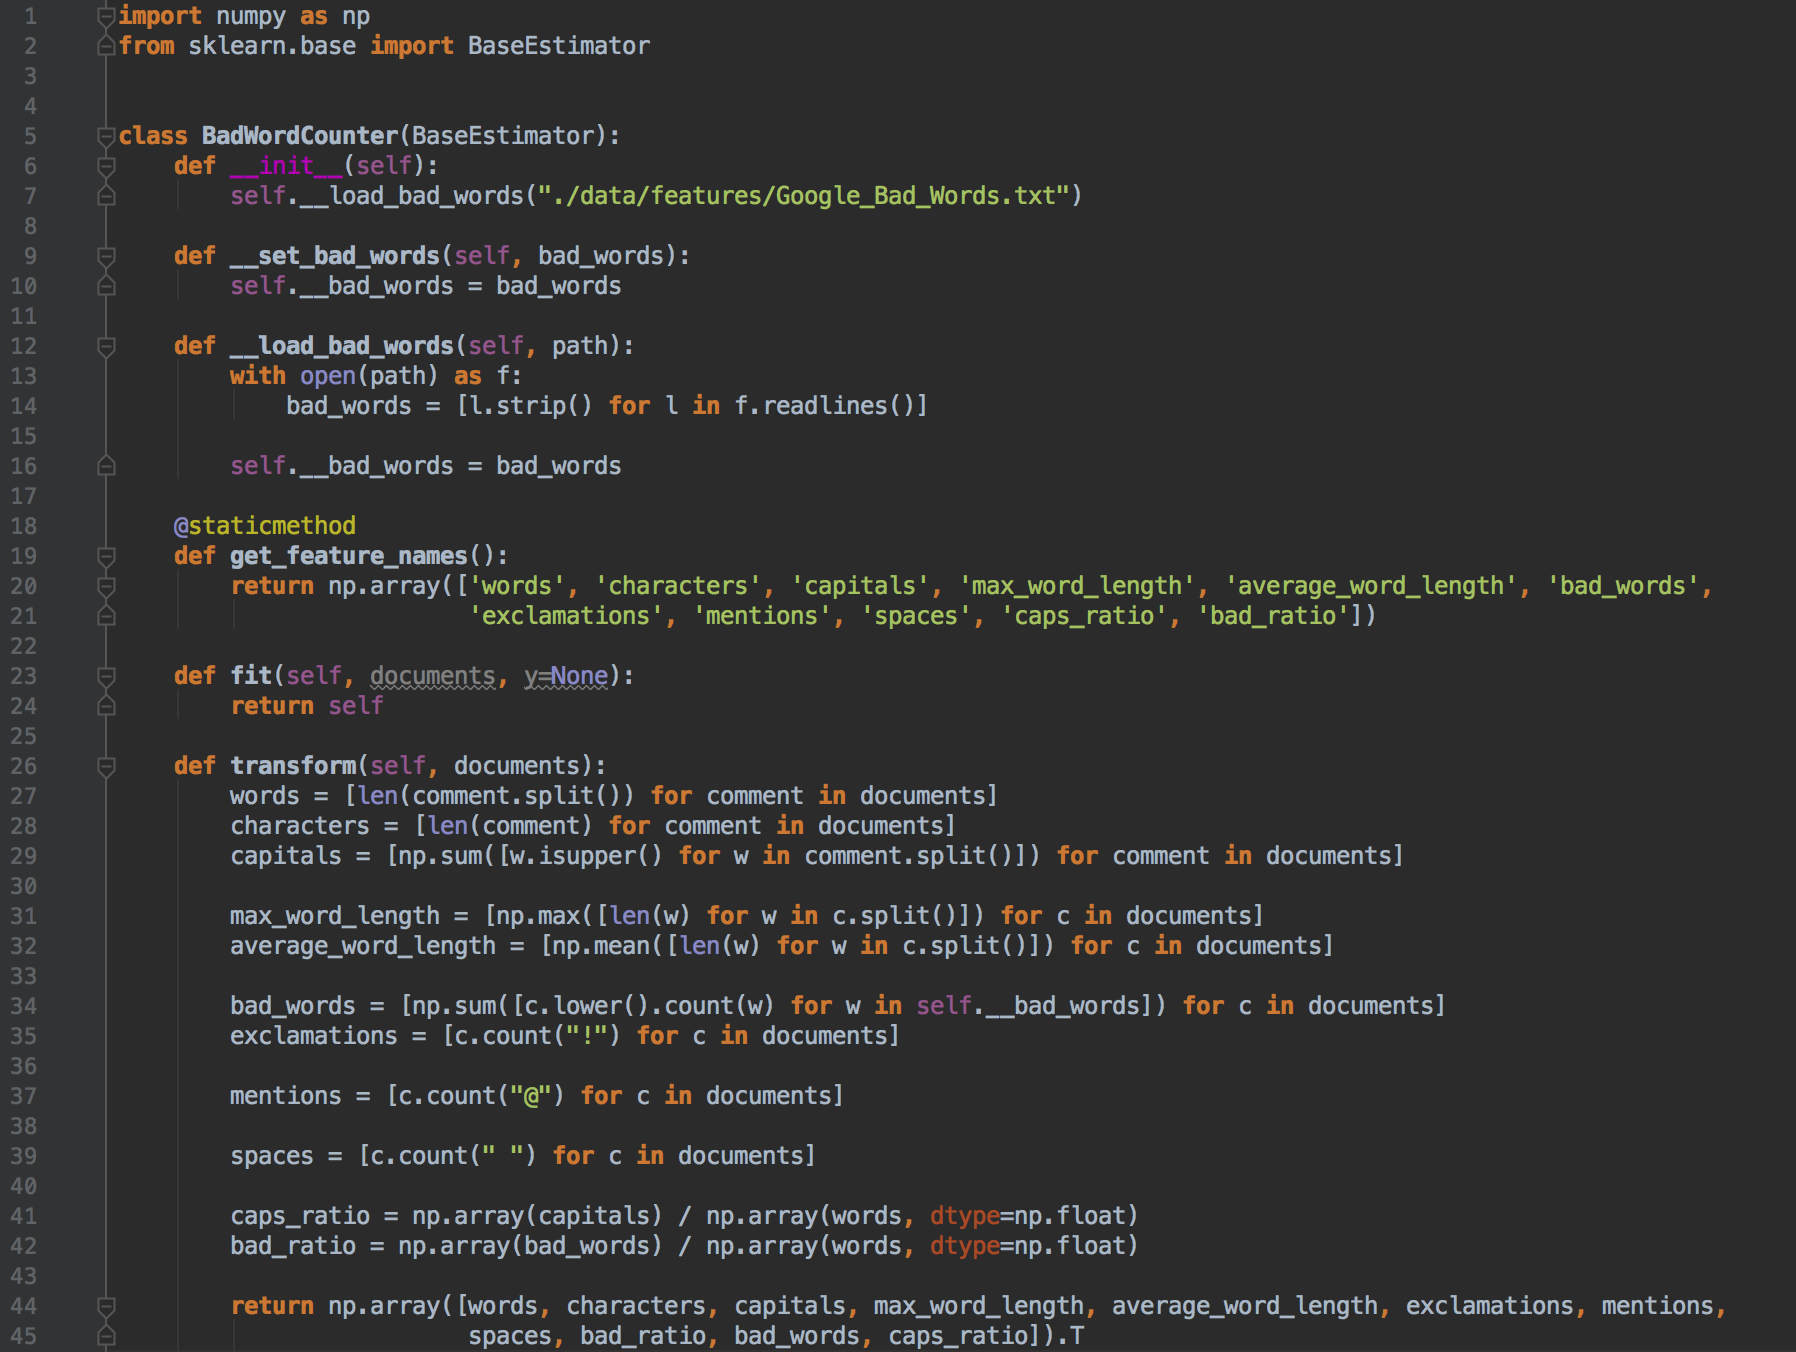
\includegraphics[width=\textwidth]{Images/Implementation/DataProcessing/AbuseDetection/BadWordCounter}
    \caption{Bad Word Counter feature engineering class.}
    \label{fig:AbuseDetection-BadWordCounter}
\end{figure}

\paragraph{Bad Word Counter} This feature engineering technique takes advantage of a list of the commonly used ``inappropriate'' words. The list was originally developed by Google for their ``What do you love'' project \cite{GitHub:GoogleBadWordList}. It contains 451 words which Google considered inappropriate and banned from being displayed on the project. The transformation was implemented using a new class which uses the \emph{BaseEstimator} interface, more specifically, the fit and transform methods of the \emph{BaseEstimator}. As applying this transformation results in a completely new set of features which are independent for every sample, the fit method is not necessary and is therefore not actually implemented. There are currently eleven unique features generated, some more important than others but this is up to the classifier to decide. All the features returned are numerical (either integer or float).

The class starts by loading the Bad Words List (BWL), in the constructor, when the class is instantiated. The \emph{transform} function accepts a list of documents (comments) and returns a two-dimensional array with $|documents| \times |features|$ elements. Lines 27, 28, 29 compute the number of words, characters and uppercase words in each comment. Lines 31 and 32 then proceed to compute the length of the longest word and the average word length for each comment. These features are pretty generic and do not necessarily indicate any abusive comments but the model may find a pattern so we can include them for safety. The next features generated are the number of bad words based on the BWL and the number of exclamation marks in each comment. These two features are quite indicative of an abusive comment. Next, we compute a few more generic features including the number of mentions (users) and the number of spaces. Lastly, we compute the caps to non-caps ratio and the bad to normal words ratio and represent them as floats to indicate the severity of post. Finally, we combine all these features and return a 2D matrix.

\paragraph{TFIDF Vectoriser} This process involves converting a collection of raw documents to a matrix of TF-IDF features. It is equivalent to using a CountVectorizer followed by TfidfTransformer \cite{Scikit:TFIDFVectorizer}. 

The CountVectorizer in the \emph{scikit-learn} package generates features by tokenising strings giving an integer id for each possible token, counting the occurrences of tokens in each document, and then normalising and weighting with diminishing importance tokens that occur in the majority of documents \cite{scikit:tfidf}. We call vectorisation the general process of turning a collection of text documents into numerical feature vectors. This specific strategy (tokenisation, counting and normalisation) is called the Bag of Words or ``Bag of n-grams'' representation. Documents are described by word occurrences while completely ignoring the relative position information of the words in the document \cite{scikit:tfidf}.

In large comments, some words will appear very often (e.g. ``the'', ``a'', ``an'', etc). These words are known as stop words and have very little meaning in terms of the classification process. Feeding these terms directly into the classifier would result in them overshadowing the less frequent, but more meaningful terms. TF means term-frequency while TF-IDF means term-frequency times inverse document-frequency \cite{scikit:tfidf}. The TF-IDF transformer simply re-weights the count features into floating point values, suitable for usage by a classifier, by multiplying the term frequency with the IDF component. The IDF component can be computed using equation \ref{equation:IDF}, where $n_{d}$ is the total number of documents, and $df(d,t)$ is the number of documents that contain term $t$. The resulting TF-IDF vectors are then normalised by the Euclidean norm.

\begin{equation}
    idf(t) = log\frac{1 + n_{d}}{1 + df(d, t)} + 1
    \label{equation:IDF}
\end{equation}

Two separate set of TF-IDF features were generated, one for words and one for characters. The \textit{analyser} can be tweaked which determines whether the feature should be made of word or character n-grams. The \textit{ngram\_range} parameter takes a lower and upper boundary of the range of n-values for different n-grams to be extracted. All values of n such that $min\_n <= n <= max\_n$ will be used. The \textit{binary} value of $False$ ensures that frequencies of zero are not normalised to one.

\begin{figure}[H]
    \centering
    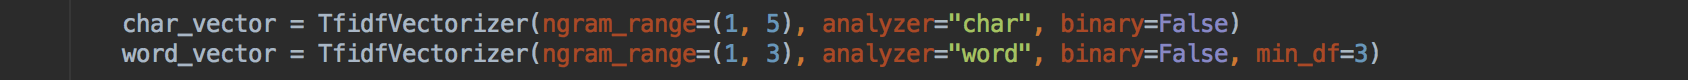
\includegraphics[width=\textwidth]{Images/Implementation/DataProcessing/AbuseDetection/TFIDF}
    \caption{Generating character and word ngram frequencies.}
    \label{fig:AbuseDetection-TFIDF}
\end{figure}

\subparagraph{Characters} The character vectoriser uses the character analyser to generate n-grams for different combinations of characters in the comment. This vectoriser uses a \textit{ngram\_range} of 1-5, extracting character sequences at least one character long.

\subparagraph{Words} The word vectoriser uses the word analyser which produces tokens on delimiters, such as white spaces and punctuation. Additionally, it uses an \textit{ngram\_range} of 1-3. The main difference here is that this uses a \textit{min\_df} value of 3, producing a vocabulary ignoring terms that have a document frequency strictly lower than the given threshold.

\paragraph{Feature Stacking}
As multiple feature engineering techniques were used, and each technique required the raw comments to generate the features, these techniques could not just simply be pipelined. Each of these techniques produced a different set of features as output, meaning that the output of one transformation could not be used as the input of another technique. In order to resolve this issue, a \textit{FeatureStacker} class was built to stack the output of multiple techniques. The class takes a list of estimators as inputs to produce a generic estimator. The \textit{FeatureStacker} implements the fit and transform methods from the base estimator. The fit method simply calls the same procedure on all estimators in the list, thus fitting each estimator to the raw comments. The transform method then applies each of the transformation, horizontally stacking the set of features returned by each transformer, returning the generated compressed sparse row matrix \cite{Scipy:ToCSR}.

\begin{figure}[H]
    \centering
    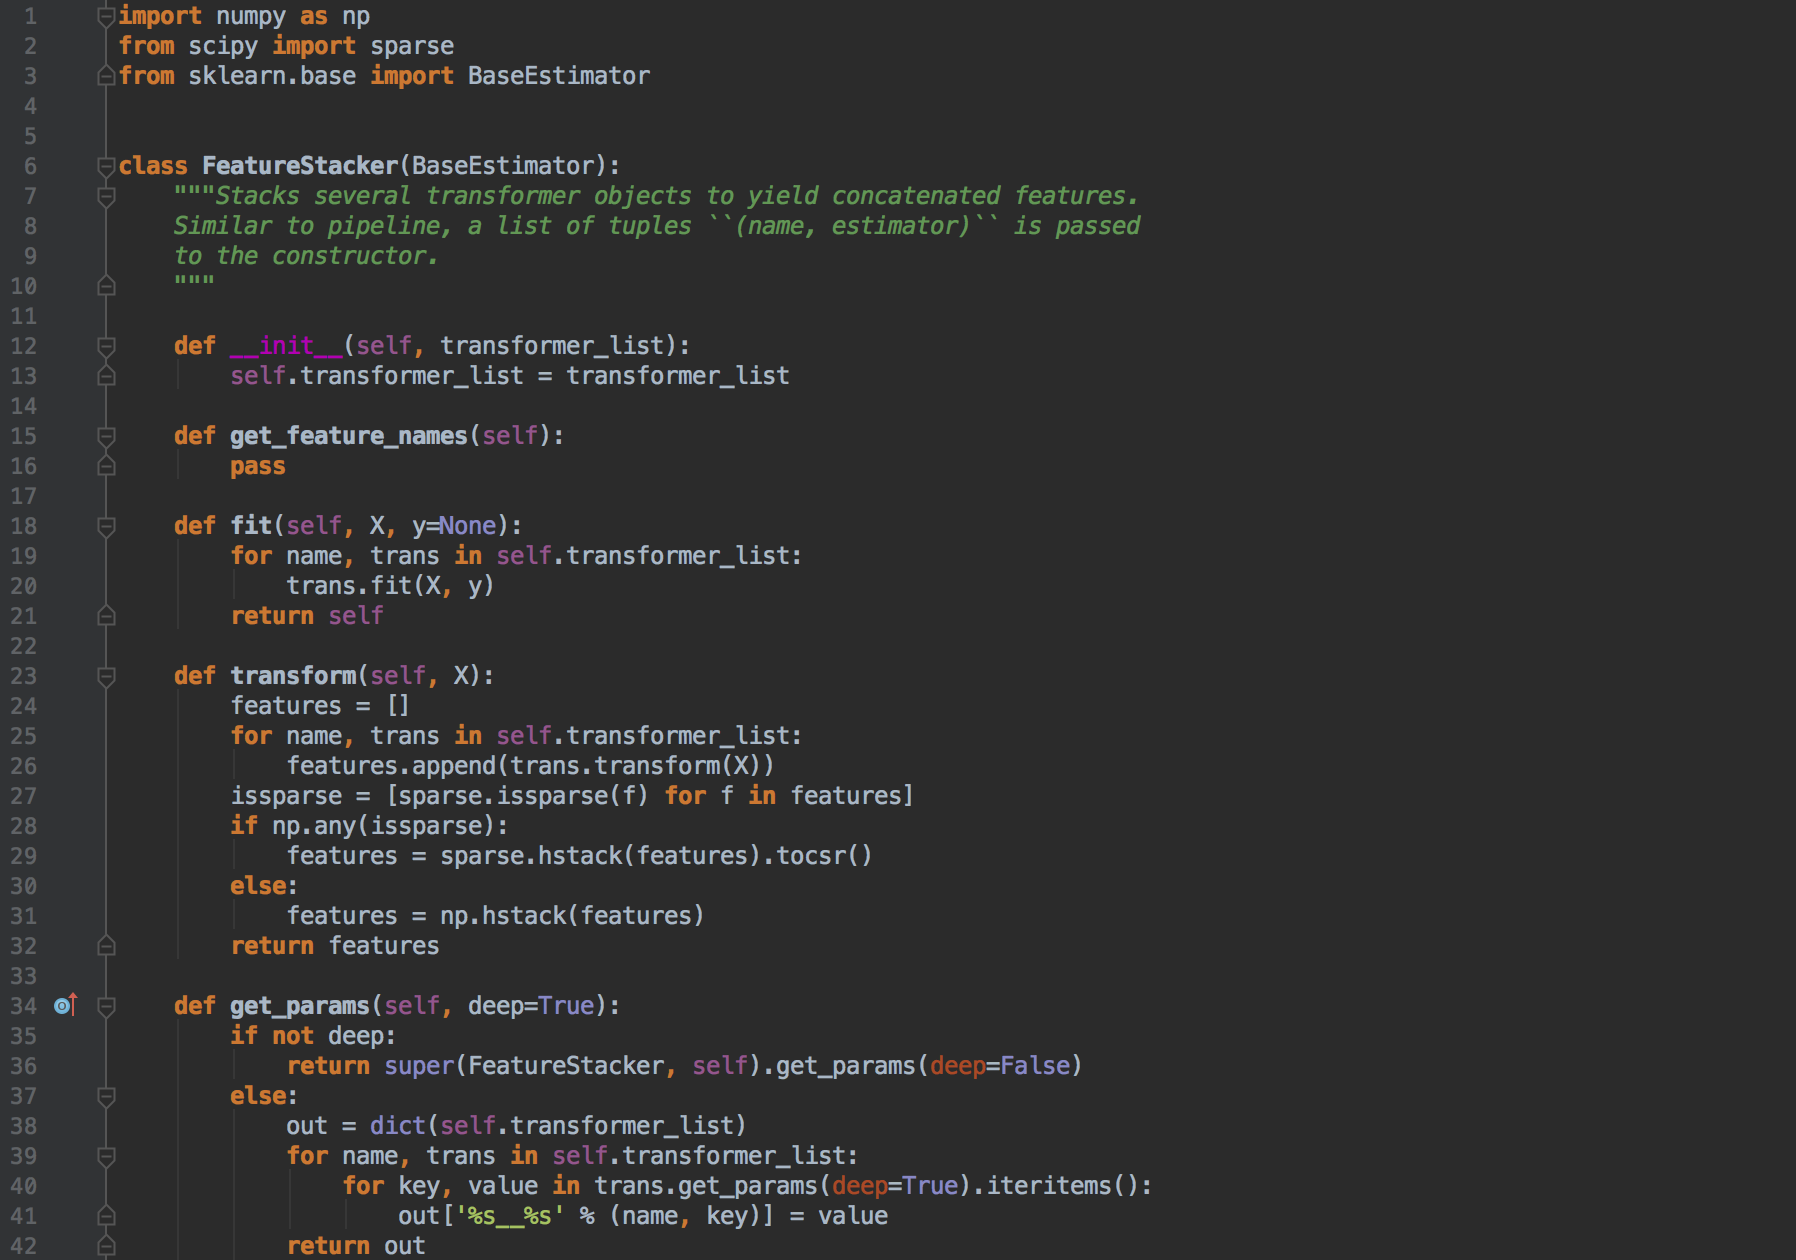
\includegraphics[width=\textwidth]{Images/Implementation/DataProcessing/AbuseDetection/FeatureStacker}
    \caption{The Feature Stacker class for combining multiple features.}
    \label{fig:AbuseDetection-FeatureStacker}
\end{figure}

\subsubsection{Feature Selection}
Not all the features generated by the feature engineering techniques above are useful to the classifier. It's hard to tell by manual inspection which of these features will be good and which will be bad. Univariate feature selection works by selecting the best features based on univariate statistical tests. It can be seen as a preprocessing step to an estimator \cite{Scikit:FeatureSelection}. The chi-squared test is one such statistical test, measuring dependencies between stochastic variables. This score can be used to select the \emph{n\_features} with the highest $\chi^2$ values for the chi-square statistic test on X, which must contain only non-negative features such as booleans or frequencies, relative to the classes. Using the \textit{SelectPercentile} package with the chi-squared scoring function we can remove features that are the most likely to be independent of class and therefore irrelevant for classification \cite{Scikit:SelectPercentile, Scikit:ChiSquared}. After playing with various different parameters, the top 16\% of the features were kept, as demonstrated in figure \ref{fig:AbuseDetection-Modelling}.

\subsubsection{Modelling}
There are various different machine learning models available, ranging from regression to classifiers to neural networks, each with their own advantages and disadvantages. In order to find the best solution, multiple models were used and tested before settling for one model. The three models generated were: Logistic Regression (LR), Supper Vector Machine (SVM) and Stochastic Gradient Descent Classifier (SGD).

\begin{figure}[H]
    \centering
    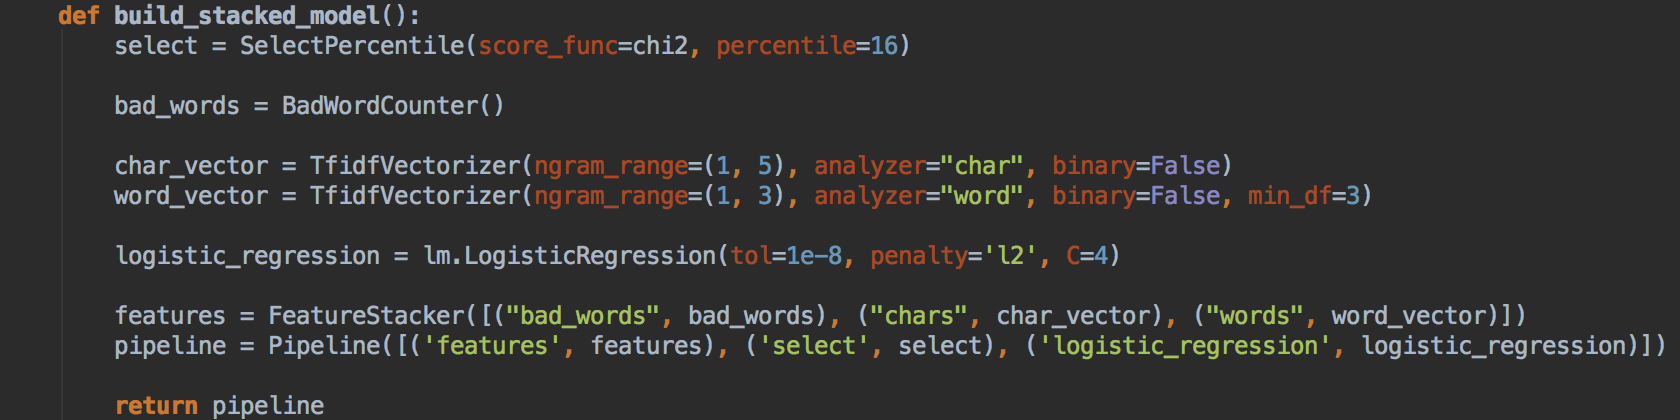
\includegraphics[width=\textwidth]{Images/Implementation/DataProcessing/AbuseDetection/Modelling}
    \caption{Function that cleans a post}
    \label{fig:AbuseDetection-Modelling}
\end{figure}

Besides the classifier used, the modelling process was essentially the same throughout all models. Figure \ref{fig:AbuseDetection-Modelling} shows the code for creating a Linear Regression model. The function simply creates a pipeline with the feature stacker containing all the feature transformers, the feature selection function using the chi-square test and the appropriate classifier. The process for training this classifier and finding the best parameters is discussed further in this section.

\begin{figure}[H]
    \centering
    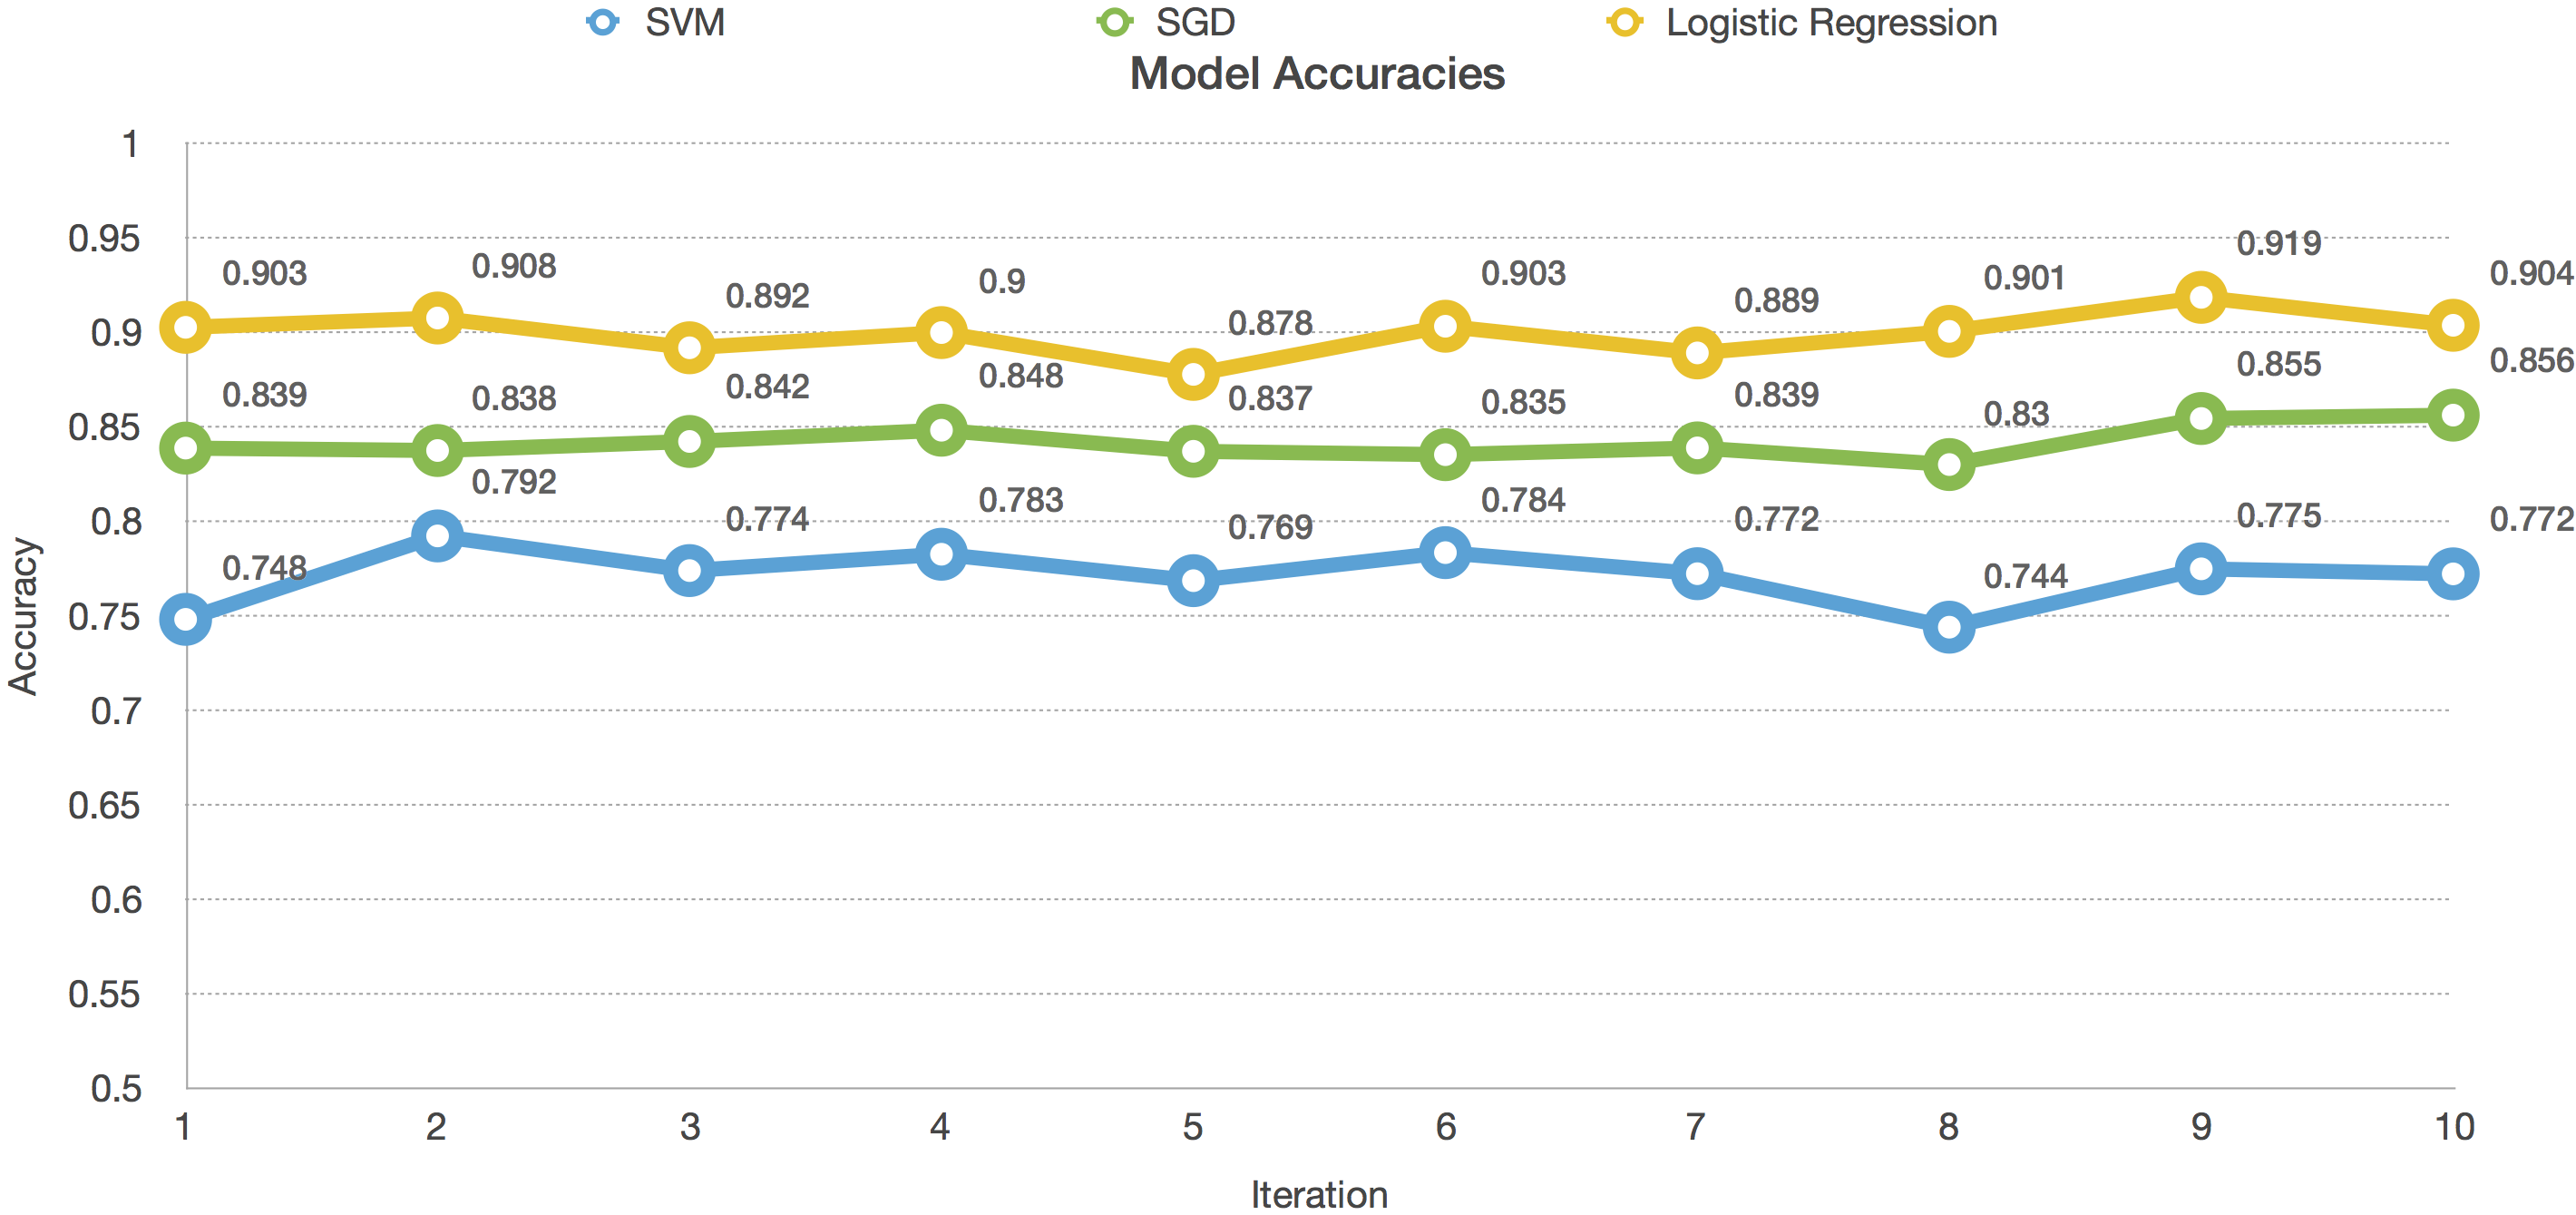
\includegraphics[width=\textwidth]{Images/Implementation/DataProcessing/AbuseDetection/ModelAccuracies}
    \caption{Accuracies for 3 model across 10 different iterations.}
    \label{fig:AbuseDetection-ModelAccuracies}
\end{figure}

The graph in figure \ref{fig:AbuseDetection-ModelAccuracies} shows the accuracies achieved by the three models across ten different iterations. As visible in the graph, the Logistic Regression performs significantly better than the other models. SVM performed lower than expected but this could be a result of the parameters used, as the accuracy of an SVM model is highly dependent on it's tuning parameter \textit{C}. Logistic Regression was used as the final model for predictions.

\subsubsection{Training}
Scikit-Learn provides a utility for exhaustively testing models with a list of values for each parameter. The \textit{GridSearchCV} package takes a \textit{BaseEstimator} as input along with a dictionary of parameters where the key represents the name of the parameter and the value is the list of values to test for that parameter \cite{Scikit:GridSearch}. When fitted, the package fits the estimator to the data with all possible combinations of parameters from the dictionary and evaluates the prediction using cross-validation and a scoring method. Once it has finished executing, it returns the best set of parameters for the model (i.e. the highest scoring parameters) which can be used to create a single instance of the estimator. This is demonstrated in figure \ref{fig:AbuseDetection-Training} where the SVM pipeline is used, along with the Area Under the Curve (AUC) scoring function, to tests different values of \textit{C} for two different kernels.

\begin{figure}[H]
    \centering
    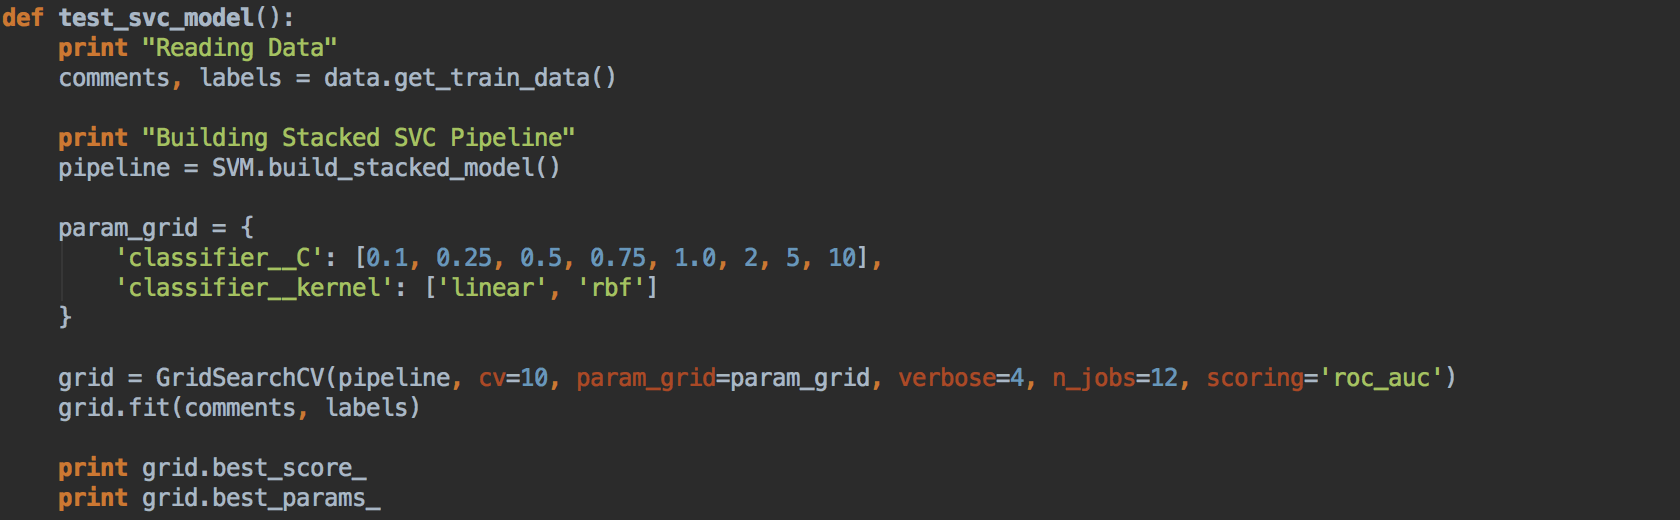
\includegraphics[width=\textwidth]{Images/Implementation/DataProcessing/AbuseDetection/Training}
    \caption{Function for testing an estimator and finding best parameters.}
    \label{fig:AbuseDetection-Training}
\end{figure}

\subsubsection{Exporting} \label{sec:exporting}
With the models trained and the best parameters discovered, a single instance of the model fitted to the entire training dataset can be created and saved to a file. This allows the model to be reloaded quickly, with the same settings and information, to make predictions. The function in figure \ref{fig:AbuseDetection-Exporting} generates an instance of the pipeline with a linear regression model. The pipeline is fitted to the training data, evaluated using the test data and the resulting estimator is stored to a file.

\begin{figure}[H]
    \centering
    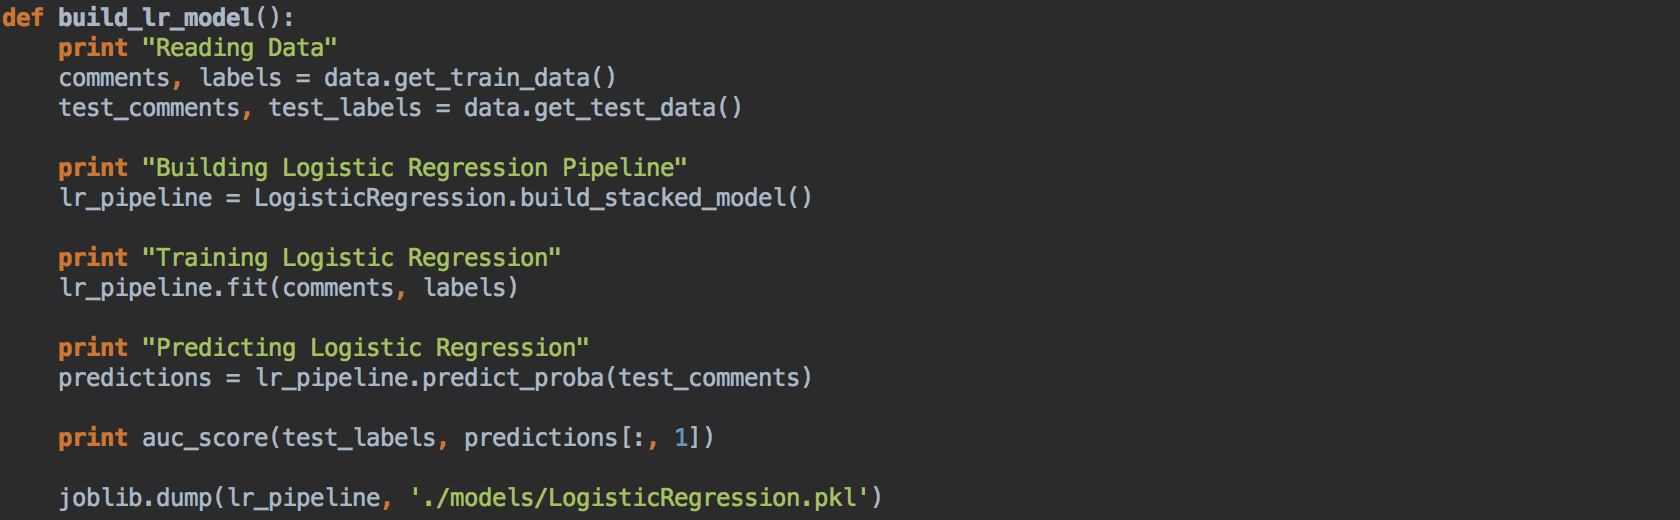
\includegraphics[width=\textwidth]{Images/Implementation/DataProcessing/AbuseDetection/Exporting}
    \caption{Function for exporting a Linear Regression model.}
    \label{fig:AbuseDetection-Exporting}
\end{figure}

\subsubsection{Predicting}
A separate script was created to make predictions on comments. It can be executed with an optional command line argument, \textit{reported}, once a model has been exported. The script firstly loads the exported model into memory and then proceeds to load the comments from the database. To interact with the database, a custom MySQL wrapper class was created. The \textit{reported} parameter is used when deciding which comments to load for processing. If the parameter is set to false, the default value, then all comments made in the last 24 hours are loaded using the query in figure \ref{fig:AbuseDetection-DailyComments}. This is because the script is designed to run on a daily basis and hence any comments older than a day should already have been processed in the last iteration. If the parameter is set to true then only comments which have been reported but not yet processed are loaded using the query in figure \ref{fig:AbuseDetection-ReportedComments}. This option is supported so that reported comments can be processed more frequently.
\begin{figure}[H]
    \centering
    \begin{subfigure}[t]{\linewidth}
        \centering
        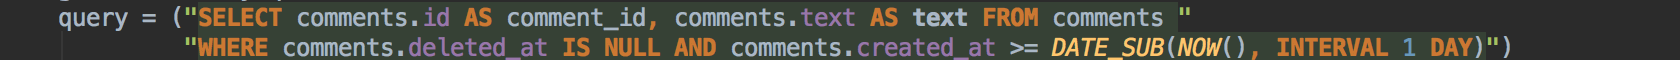
\includegraphics[width=\linewidth]{Images/Implementation/DataProcessing/AbuseDetection/DailyCommentsQuery}
        \caption{Comments made in the last 24 hours.}\label{fig:AbuseDetection-DailyComments}        
    \end{subfigure}
    \quad
    \begin{subfigure}[t]{\linewidth}
        \centering
        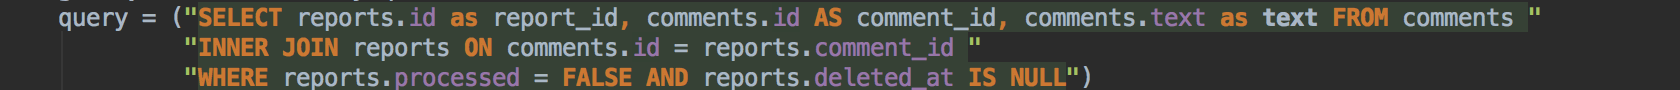
\includegraphics[width=\linewidth]{Images/Implementation/DataProcessing/AbuseDetection/ReportedCommentsQuery}
        \caption{Reported comments.}\label{fig:AbuseDetection-ReportedComments}
    \end{subfigure}
    \caption{Fetching unprocessed comments from the database.}\label{fig:AbuseDetection-LoadingComments}
\end{figure}

Once the comments are loaded, their class probabilities are predicted and multiplied by 100 to produce an abuse rating. The resulting predictions are then used to update the comments in the database with their abuse rating. If the reported comments have been loaded then all associated reports for the processed comments are marked as processed. Figure \ref{fig:AbuseDetection-UpdatePredictions} shows the function used to achieve this. After the queries have been executed, we can close the cursor and MySQL connection to reduce the load on the database.

\begin{figure}[H]
    \centering
    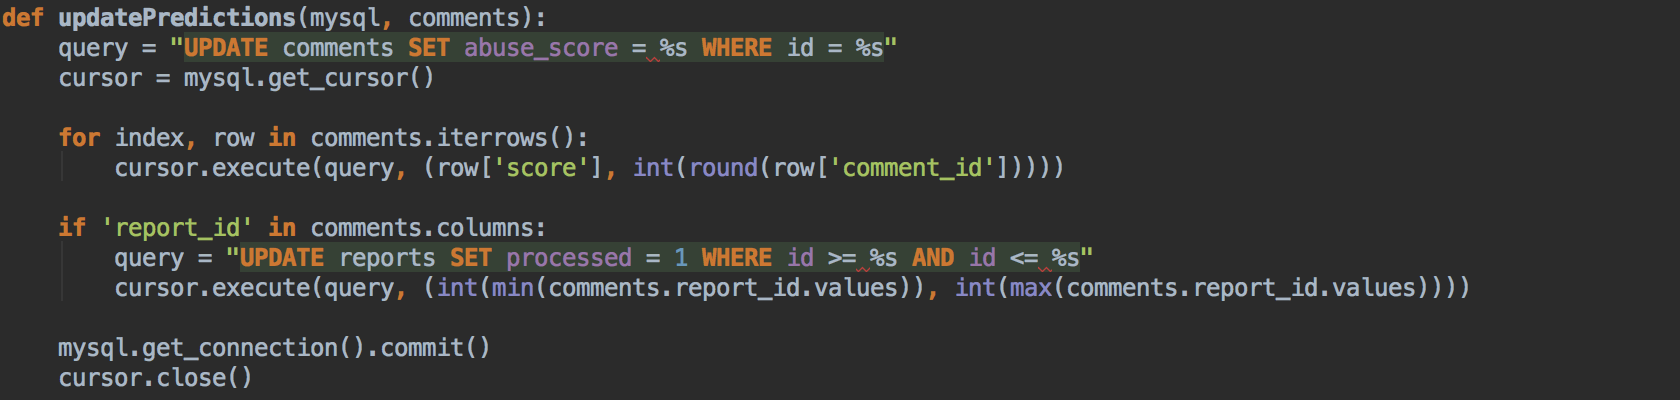
\includegraphics[width=\textwidth]{Images/Implementation/DataProcessing/AbuseDetection/UpdatingScores}
    \caption{Function for updating the abuse rating of comments in the database.}
    \label{fig:AbuseDetection-UpdatePredictions}
\end{figure}